\documentclass{article}
\usepackage[utf8]{inputenc}
\usepackage{csquotes}
\usepackage[english]{babel}
\usepackage{appendix}
\usepackage{multicol}
\usepackage{titlesec}
\usepackage[nottoc]{tocbibind}
\usepackage{listings}
\usepackage{multicol}
\usepackage{titling}
\usepackage{graphicx}
\usepackage{tabularx}
\usepackage{float}
\usepackage{arydshln}
\usepackage{soul}
\usepackage{amsmath}
\usepackage{enumitem}
\usepackage{natbib}

\setcounter{tocdepth}{4}
\setcounter{secnumdepth}{4}

\titleformat{\paragraph}
{\normalfont\normalsize\bfseries}{\theparagraph}{1em}{}
\titlespacing*{\paragraph}
{0pt}{3.25ex plus 1ex minus .2ex}{1.5ex plus .2ex}

\newcommand{\subtitle}[1]{%
\posttitle{%
\par\end{center}
\begin{center}\large\textit{#1}\end{center}
\vskip0.5em}%
}
\bibliographystyle{agsm}


\title{What is required by software platforms in order to give a good developer experience?}
\subtitle{A Case Study in Qlik Core's Developer Experience}
\author{Christoffer MacFie}
\date{January 2019}

\begin{document}
\maketitle
\newpage
\tableofcontents
\newpage

\section{Background and Purpose}

This paper aims to

\subsection{What is User Experience?}

User Experience (UX) is the collective term of many disciplines merged
into one that evaluates the overall experience delivered to a user of a
system, product or service. The term was coined by Donald Norman in the
1990s[Citation needed] who has a background in the fields of cognitive
science and usability engineering. It is defined by ISO 9241-210, part
of "Ergonomics of human system interactions", as \begin{quote}
"a person's perceptions and responses that result from the use or anticipated use of
a product, system or service"
\end{quote}
It can therefor be considered a
subjective quality of a product, system or service.

More text here...
\subsection{What is Developer Experience?}

Developer Experience, or DX, is similar to the more well known User
Experience (UX), but with the user being a software developer. DX is
defined by Sam Jarman as

\begin{displayquote}
"The experience developers have when they use your product, be it
client libraries, SDKs, frameworks, open source code, tools, API,
technology or service."\cite{jarman}
\end{displayquote}

More text here ...


\subsection{How do we define 'Good DX'?}

There are many potential factors for defining what constitutes 'Good'
DX. The website EveryDeveloper\cite{everydeveloper} has developed a \textit{DX Index} from
1-10, where they consider four factors:

\begin{enumerate}
\item Are the libraries available in popular languages?
\item How prominent, in-depth are the starting guides?
\item Are the solutions self-serving, without need of demos or 'call us'?
\item Is the pricing clearly stated?
\end{enumerate}



Sam Jarman has other factors for he uses to evaluate
if something gives a good DX. He for example puts emphasis on
communication between the product provider and the developer.\cite{jarman} The dialog
between the product provider and the community needs to be authentic,
open and honest in order the give a good developer experience, according
to Jarman.
\\ \\
It has been researched what makes a developer
happy and unhappy\cite{unhappy}, and found several indicators. They found both
internal- and external factors, where external are the most interesting
for this project. However, the internal unhappiness factor of 'work
withdrawal' is worth noticing. Being stuck on a task without any
progress for too long leads to unhappiness.

More text here ...

\subsection{What is Qlik Core?}

Qlik Core (QC) is, as described on the official website, "an analytics
development platform built around Qlik Associative Engine and
Qlik-authored open source libraries".\cite{qlikwebsite} The
platform consists of several components, with it's central part being
the engine. The platform also provides 'Mira', a software to generate
insights about the data. Furthermore, it provides the two javascript
libraries 'Halyard' and 'Enigma'. Halyard helps the user to easily load
in data into the engine. Enigma helps the user communicate with the
engine.


\subsection{Standardisation}
International Organisation for Standardization (ISO) has yet to present a
standard for developer experience. There are however other standards from ISO
that are interesting to have a look at. One is \textit{ISO 9126 Software engineering - Product Quality}.
One part of the ISO-standard concerns quality. This part of the ISO standardizes how to measure the quality of software.
It has six different characteristics: functionality, reliability, usability, efficiency, maintainability and
portability. Each of these characteristics have sub-characteristics. The definition of each
characteristic is listed, and their sub-characteristics, is in table \ref{tabl:standard1} and table \ref{tabl:standard2}


\begin{table}[H]
\centering
\begin{tabularx}{\columnwidth}{|l|l|X|}
\hline

\multicolumn{3}{c}{\textbf{Functionality}} \\ \hline
F1  &   Suitability &The capability of the software product to provide an appropriate set of
functions to specified tasks and objectives \\ \hline
F2  &   Accurateness &  The cap... / / ... to provide the right or agreed results or effects with the needed
degree of precision \\ \hline
F3  &   Interoperability& The cap... / / ... to interact with one or more specified systems \\ \hline
F4  &   Security& The cap... / / ... to protect information and data so that unauthorised persons or systems
cannot read or modify them and authorised persons or systems are not denied access to them \\ \hline

\multicolumn{3}{c}{\textbf{Reliability}} \\ \hline
R1  & Maturity    & The cap... / / ... to avoid failure as a result of faults in the software \\
\hline
R2  &   Fault tolerance & The cap... / / ... to maintain a specified level of performance in cases of the
software faults or of infringement of its specified interface \\ \hline
R3  &   Recoverability  & The cap... / / ... to re-establish a specified level of performance and recover the
data directly affected in the case of a failure \\ \hline

\multicolumn{3}{c}{\textbf{Usability}} \\ \hline
U1  &   Understandability   &   The cap... / / ... to enable the user to understand whether the
software is suitable, and how it can be used for particular tasks and conditions of use \\ \hline
U2&Learnability & The cap... / / ... to enable the user to learn it application \\ \hline
U3&Operability & The cap... / / ... to operate and control it \\ \hline
U4&Attractiveness& The cap... / / ... to be attractive to the user [visually] \\ \hline

\multicolumn{3}{c}{\textbf{Efficiency}} \\ \hline
E1&Time Behaviour & The cap... / / ... to provide appropriate response and processing times and
throughput rates when performing its function, under stated conditions \\ \hline
E2&Resource Utilisation & The cap... / / ... to use appropriate amounts and types of resources when the software
performs its function under stated conditions \\ \hline
\end{tabularx}
\caption{Part 1: ISO-9216}
\label{tabl:standard1}
\end{table}

\begin{table}[H]
\centering
\begin{tabularx}{\columnwidth}{|l|l|X|}
\hline
\multicolumn{3}{c}{\textbf{Maintainability}} \\ \hline
M1&Analysability & The cap... / / ... to be diagnosed for deficiencies or causes of failures in the
software, or for the parts to be modified to be identified \\ \hline
M2&Changeability & The cap... / / ... to enable a specified modification to be implemented \\ \hline
M3&Stability & The cap... / / ... to avoid unexpected effects from modifications of the software \\ \hline
M4&Testability &The cap... / / ... to enable modified software to be validated \\ \hline

\multicolumn{3}{c}{\textbf{Portability}} \\ \hline
P1& Adaptability &The cap... / / ... to be adapted for different specified enviroments without applying
actions or means other than tose provided for this purpose for the software considered \\ \hline
P2&Installability& The cap... / / ... to be installed in a specified environment \\ \hline
P3&Co-existence &The cap... / / ... to co-exist with other independent software in a common enviroment sharing
common resources \\ \hline
P4&Replaceability &The cap... / / ... to be used in a place of another specified software product for the same
purpose in the same environment \\ \hline

\multicolumn{3}{c}{\textbf{All characteristics}} \\ \hline
AC&Compliance & The cap... / / ... to adhere to standards and conventions relating to the
characteristic \\ \hline
\end{tabularx}
\caption{Part 2: ISO-9216}
\label{tabl:standard2}
\end{table}


There is also a standard for UX,
namely \textit{ISO-9241-210: Ergonomics of human-system interaction -
Part 210: Human-centred design for interactive systems}.

More text here ...
\subsection{Kinds of APIs}

Application Program Interfaces (APIs) are, simply put, a software that
lets one application interact with another application's inner data and
services. Applications are in need of an interface to interact with it's
inner parts to create, read, update and read (CRUD) as well as execute
commands. APIs provide this link between the two pieces of software that let's
them communicate.Because of APIs broad nature, there are many types of
APIs.

\subsubsection{Internal, Public and Partner APIs}
APIs have different level of openness, depending on who is going to access them. They are
usually divided into three groups: Internal APIs, Public APIs and Partner APIs. These
three groups are explained below.
\paragraph{Internal APIs}
Internal APIs are APIs that har meant to be used in production and
within an organisation or company. They are often developed to be used
between different teams in the company to be able to connect software
components in the application, without having to actually know the code
of the component. The benefit of this is that the team can open up certain
needed functionality of the software to other teams while still being in
control of their own code. This kind of APIs are protected and require
internal API keys to access to ensure that people outside of the company
are not able to access them.
\paragraph{Public APIs}
Public APIs is another kind of API. This is a way for the company to
open up functionality of the software's inner workings to the world so
that anyone may build new applications that are built upon the original
software. This kind of interface often only has a small percentage of
the functionality that the internal API has, since the circuitry of the
software must be protected for security reasons as well as from business
intelligence theft. If the internal API was open to the public anyone
could build their own copy of the program. These kind of APIs either do
not require any API key to access, or have an API key that is open for
anyone to acquire (either through payment or for free).
\paragraph{Partner APIs}
Partner APIs are a third interface that can be shared
business-to-business (B2B), with strategic partners to the company.
Partner APIs often put some restraints on what can be exposed so that
the inner workings of the software is still protected, but is able to be
more open than a public API. These kinds of APIs require an API key that
is often contracted with terms and condition to protect the company's
business intelligence.\cite{levin}

\subsubsection{Web APIs}

When using services over the internet, there are many different protocols that can be used to communicate.
And just like with many other things in computer science, there are many valid approaches whom all have their
pros and cons. The world wide web (WWW) is largely built upon the application protocol
hypertext-transfer-protocol (HTTP) which, amongst other things, provides CRUD (Create, Retrieve, Update, Delete)
methods to be applied on resources. Resources in this context is refers to any \textit{thing}: file, object, document,
text, etc, that is provided by a web service. There are however many ways of utilizing this protocol to let a
client access and manipulate server-side data, as well as execute commands. Below we describe two methods.

\paragraph{REST}

Representational State Transfer (REST) is a software architectural style
that is used in web services which acts as a communication bridge
between computer systems and the internet. It let's the system interact
and manipulate the service it's interacting with. REST solves many
issues that had been present in previous implementations of
communication between computer systems and the web.
\\ \\
One of the key factors in REST is that it's stateless. Statelessness in
this context means that the two communicating parties does not need to
know anything about each other or have seen previous messages to
understand future ones. This feature is possible by limiting it to the
use of resources instead of commands. REST-APIs can therefor not ask the
server side to execute a specific custom command, but is limited to
using CRUD methods.
\\ \\
A REST request consists of an HTTP method, a header containing
information about the request, the path to the resource and lastly and
optional message body consisting of data.\cite{rest1}\cite{rest2}
\\ \\
Statelessness makes it possible to separate the client and the server.
Code changes to the server will not require changes to the client's
code, and vice versa, as long as the message format between the two are
kept the same.
\\ \\
Since REST does not use sessions, but simply responds to any incoming
requests, it's easy to scale up. It simply requires more bandwidth and
processing power to be able to handle more requests per second.
\\ \\
If you want to for example post a message as a user with the \texttt{userID 1}, it
could look something like this when using REST:

\begin{lstlisting}
POST /users/1/messages HTTP/1.1
Host: example.com
Content-Type: application/json
{"msg": "Test123"}
\end{lstlisting}

Here, the resource of \texttt{/users/1/messages} is fetched and then the
new message is created and put there. The server does not work in
sessions and cannot tell clients that a new message is available. The
clients has to periodically ask the server if there are any new messages
to retrieve.
\\ \\
REST may be appropriate to use when you mostly want to do CRUD-commands
or manipulate data.

\paragraph{RPC}

%    https://en.wikipedia.org/wiki/Remote_procedure_call
%    https://www.smashingmagazine.com/2016/09/understanding-rest-and-rpc-for-http-apis/
Remote Procedure Call (RPC) is a protocol used to execute commands on remote systems. RPC is, like REST, also
built on HTTP, but uses mostly just the \texttt{GET} and \texttt{POST} commands. RPC is a request-response protocol and is, unlike
REST, stateful. Ergo, the protocol works with sessions between a client and a server, and previous messages may
be needed in order to understand future ones.
\\ \\
An upside of RPC is that it let's a client request the server to execute
a custom command. Making an RPC-call is much like making a normal
function call, in that you simply provide the name of the method and the
parameters. A consequence of this is that code changes on server-side,
such as method-name or parameter input, may require code changes on the
client side as well.
\\ \\
Since RPC has two-way communication, the server can tell the client when
something has changed, whereas in REST-based communication the client
has to ping the server to check if there are any changes. An RPC based
server needs to have a unique session for each client, which can cause
problems with scalability.
\\ \\
If we go back to example used in the previous section: posting a message
may look something like this:

\begin{lstlisting}
POST /SendMessage HTTP/1.1
Host: example.com
Content-Type: application/json
{"userId": 1, "msg": "Test123"}
\end{lstlisting}

Here, the server has a custom method called \texttt{SendMessage}. If the
method call is not made asynchronous, the client is put in wait until
the server responds with an acknowledgement or the call reaches a
timeout. Since RPC uses sessions and custom commands, the method can be
implemented as such that other sessions should be notified that a new
message has been sent, and the server can send it out to appropriate
clients.
\\ \\
RPC may be appropriate to use when you have functionality that can
benefit from two-way communication or is mainly command-oriented.

\subsubsection{What type of API is Qlik Core?}

Qlik Core consists of several components which utilizes different types
of APIs. Since Qlik Associative Engine is mostly action based, it uses
JSON-RPC: a remote procedure call protocol in JSON format. Qlik Core
also provides a discovery service called Mira, which let's the user make
insights about their data. Mira is a REST-API, since this is a about
retrieving data and not performing actions.\cite{qlikwebsite}

\subsection{API User Personas}
There are many types of people using platforms, whom all have different
requirements. They can be roughly divided into two important groups:
'Decision makers' and 'Users'. These both need to be catered to in order
to have a successful platform: if the decision makers are ignored the
platform will not be implemented by companies in the first place. If the
users are ignored, the platform will be quickly dropped since it's usage
is not good enough.
\\ \\
Mark Nottingham lists 11 personas for HTTP-based APIs\cite{personas}.

More text here ...


\section{Methodology and Preparations}

There could have been many approaches to this thesis to try to find what was needed in order to find out
what people require from software platforms in order to get a good developer experience. The process we chose was to make
a survey followed by interviews to triangulate the results.

First of all we decided what aspects we were going to consider. This was followed by an inital test survey to find what
parts we wanted to investigate further. We then conducted the major survey. After that we analyzed the results and tried to find
patterns and interesting aspects. This lead to a series of questions, which we used when conducting interviews with people with
different experience and job titles. The result from the interviews were put together and related to the finding in the survey.
This finally resulted in a list of recommendation on what is needed by a software platform in order to give a good DX.

Lastly, this listed was used to analyze how well Qlik Core follow these recommendations.

\subsection{Deciding consideration aspects}

There are a lot of aspects we could have considered as requirements for
good DX. We had to limit them down however, and ended up with 14 aspects relating to software, and six aspects relating ot the
creators of software.
For the second survey, we added two more aspects, namely aspect 13 and 14 in the list below. Aspects relting to
creators of software were not part of the second survey.
The reasoning for adding two new aspects and removing aspects relating to creators is
discussed later in the paper. The fourteen original aspects were decided in a combination
of reading literature, our own experience of what we would consider when
picking software platforms, and a brainstorm meeting with more experienced
people at Qlik, consisting of an architect and developers.
The list we ended up with can be seen in table \ref{tab:aspects}.
\begin{table}[H]
\centering
\begin{tabularx}{\columnwidth}{l X}
\multicolumn{2}{c}{\textbf{List of Aspects}} \\
\hline
1    & How often the software is updated    \\
2    & I can have working code quickly  \\
3    & The API documentation gives thorough explanations on how it works    \\
4    & The API has code examples    \\
5    & The documentation doesn't assume any prior expertise \\
6    & The documentation has consistent language    \\
7    & The documentation is easy to navigate    \\
8    & The official website looks professional  \\
9    & The pricing of the software  \\
10    &  The release- and change notes are thorough \\
11   &  The software has the same features on all different platforms   \\
12    &  The software is compatible with different platforms    \\
13  &  The software is offered in more than one programming language    \\
14*    &  The software is open source    \\
15*    &  The software uses the programming language I am most comfortable with  \\
16    &  There exists an active online community around the software    \\
\hline \hline
17** & The creator of the software has good communication with it's users \\
18** & The creator of the software has high transparency with it's issues, ways of working, future plans, etc. \\
19** & The creator of the software seems professional \\
20** & The creator of the software has a good reputation online \\
21** & I have heard of the creator of the software before \\
22** & I have heard of other software the creator of the software has made
& \\
\multicolumn{2}{l}{\textit{*Not part of the first survey, **Not part of the second survey}}
\end{tabularx}
\caption{List of aspects considered to give good DX}
\label{tab:aspects}
\end{table}

Sam Jarman's article is the source for some of these
aspects.\cite{jarman} One of the points he makes is the importance of a great documentation.
He says the documentation should always be written as if the developer is
a beginner, which lead to aspect `5 - The documentation doesn't assume any prior expertise` in the list.
He also says great documentation is consistent, ergo it does not use different
words to mean the same thing, which lead to aspect `6 - The documentation has consistent language`.
A third aspect he says is needed for great documentation is that is has a
logical structure, which lead to aspect `7 - The documentation is easy to navigate`.
The last part he considers important for a great documentation is verbosity.
As he puts it, "You can never say too much". This resulted in `3 - The API documentation gives thorough explanations on how it works`.
Jarman also think it's important to have good release notes. He goes on
to present what release notes should consist of. According to him, not
only should the release notes consist of the expected, such as what's new,
updated, deprecated, fixed, etc, but also point out possible risks of the new release,
such as things that might break with it. Although these sub-features of release notes
might be interesting to list as their own aspects, we had to keep the list short
and ended up with the general aspect of `10 - The release- and change notes are thorough`.
\\ \\
Jarman also talks about pricing. He puts emphasis on that pricing of the software
should be easy to find for the developer. During the brainstorming, this
aspect was also discussed, and we ended up with the somewhat vague
aspect of `9 - The pricing of the software`. This was deliberately chosen
to be a somewhat open-ended aspect, since there's a lot of things that you can
consider around the pricing, and we simply wanted to know if pricing is something
that is often considered in general. In hindsight, it might have been better to have
divided this into several aspects, since it's difficult to know how the
survey taker interpreted the aspect.
\\ \\
When we had this short list, we sat down and thought of things that we
consider our self when picking software. The list was extended further,
with aspects related to API examples, online community and  platform compatibility.
\\ \\
After this, we had a brainstorming meeting with two senior developers and a
senior architect to further extend the list of aspects. The meeting attendees can arguably be considered
to have expertise within the field, having worked for many years within the field.
Firstly, all three
were given five minutes to write down as many aspects as they could think of.
These aspects were then presented in turn and written on a whiteboard. Any further ideas
that the three experts got when they saw the others' ideas were also added.
We then presented the list we had created ourselves earlier and the aspects not yet listed
as well on the whiteboard. The list was then discussed, as well as the phrasing of each aspect and the importance
of them.
\\ \\
Finally we ended up with the list of fourteen aspects, as seen in table \ref{tab:aspects}.
Being open source is pointed out as important by Sam Jarman, and was discussed in the meeting.
It was however not included in the final list. After the first survey was conducted, it was
also pointed out by survey takers as an aspect that they considered. It was then
added to the list to be used in the second survey.

Aspect number 15 on the list was
added for the second survey as well. The reasoning here being that the aspect
`13 - The software is offered in more than one programming language` felt
like it needed a parallel question: `15 - The software uses the programming language I am most comfortable with`,
to see if the importance of several language was solely based on the fact that
people wanted their favourite programming language.


\subsection{Linking considerations to ISO-9216-1}

As said before, there is no standard for DX. ISO-9216-1 is however a standard
to measure the quality of software, so comparing the aspects to this list can
be interesting. In table \ref{tabl:iso}, the aspects are linked to characteristics they relate to. The aspect ID's can
be found in table \ref{tab:aspects} and the references to the sub-characteristics can be seen in table \ref{tabl:standard1} and \ref{tabl:standard2}.

\begin{table}[H]
\centering
\begin{tabularx}{\columnwidth}{r|l:l:l:l:l:l}
\rotatebox{90}{\textbf{Aspect ID}}& \rotatebox{90}{\textbf{Functionality}} & \rotatebox{90}{\textbf{Reliability}} & \rotatebox{90}{\textbf{Usability}} &
\rotatebox{90}{\textbf{Efficiency}} & \rotatebox{90}{\textbf{Maintainability}} & \rotatebox{90}{\textbf{Portability}} \\ \hline
1	&		&	R1	&		&		&	M3	&	P4\\ \hline
2	&	F1, F2	&		&	U1, U2, U3	&		&	M2	&		\\ \hline
3	&	F1, F2, AC	&	AC	&	U1, U2, U3, AC	&	AC &	M1, AC	&	AC	\\ \hline
4	&	F1, F2, AC	&	AC	&	U1, U2, U3, AC	&	AC	&	M1, AC	&	AC	\\ \hline
5	&	AC	&	AC	&	U1, U2, U3, AC	&	AC	&	AC	&	AC	\\ \hline
6	&	AC	&	AC	&	U1, U2, U3, AC	&	AC	&	AC	&	AC	\\ \hline
7	&		&		&	U1, U2, U3, AC	&		&		&		\\ \hline
8	&		&		&	U4	&		&		&		\\ \hline
9	&		&		&	U1	&		&		&		\\ \hline
10	&	F1	&	R1	&	U1	&		&		&	P4	\\ \hline
11	&		&		&		&		&		&	P4	\\\hline
12	&	F3	&		&		&		&		&	P1, P2	\\ \hline
13	&		&		&	U2	&		&		&		\\\hline
14	&	AC	&	AC	&	AC	&	AC	&	M1, M2, M4, AC	&	AC	\\ \hline
15	&	F1, F2	&		&	U1, U2, U3	&		&	&		\\ \hline
16	&		&		&	U1, U2	&		&		&		\\\hline
\end{tabularx}
\caption{Relation between ISO-9216-1 and DX-aspects}
\label{tabl:iso}
\end{table}


\subsection{Quantitative vs. Qualitative data}
More text here...
\subsection{Surveys}

\subsubsection{Reasons To Do Surveys}
Surveys are a popular way to collect quantitative data.
There are several situations when surveys, or questionnaires as they are also referred to, are a good
method to use when one wants to collect quantitative data. \cite{denscombe} has described it as a good method when you are
working data that is of non-sensitive subjects, when the data sources are spread out and when the data pool is big.
He also states that questionnaires are a good way to collect data of both factual nature, as well as opinion-based.
Denscombe goes on to say that a questionnaire is likely to contain collection of both of these kinds of data and that it is
important to make it clear to the person taking the questionnaire whether or not the question is asking for an opinion, or a 'fact'.
Since this research project concerns itself with a mixture of both factual data, such as people's work experience, job titles and responsibilites, as well as opinion-based data relating to developer experience, questionnaires are a good methodology to use.

\subsubsection{Construction of a Questionnaire}
\cite{denscombe} has a section where he lays out the vital parts of a questionnaire. According to him, a questionnaire should always contain the following parts.

\begin{itemize}
\item \textbf{The Sponsor} - Clearly state who this questionnaire is from and for.
\item \textbf{The Purpose} - Why is this questionnaire being made and for what will the data be used. He warns however that one should not go into to much detail, as to lead the questionnaire taker into answering in a certain way
\item \textbf{Confidentiality} - Assert the questionnaire taker that the data collected will not be publically available or be directly linked to the him or her, if him or her so not wishes.
\item \textbf{Voluntary Responses} - Convey that the questionnaire is completely voluntary to take
\item \textbf{Thanks} - Make sure to extend your thanks to the questionnaire taker for voluntarily taking the questionnaire.
\end{itemize}

Denscombe also states that there is no good, defined number of questions that should exist in a questionnaire. However, it should be
\textit{as brief as possible}. He warns of trying to ask too many questions, for anything that \textit{might} be important. This is not a good approach. A questionnaire constructor should always try to keep the scope as tight as possible. He gives four tips for when trying to do this.
\begin{itemize}
\item Only ask questions that are absolutely vital for the research
\item Proof-read to make sure you do not ask any duplicate questions
\item Make it as fast and easy as possible to answer the questionnaire
\item Have a test-round for your questionnaire
\end{itemize}

Furthermore, Denscombe talks about phrasing of questions and knowing your target audience. He gives a comprehensive list of things to think of when doing this. Some key parts are that using words that suitable for your target audience, avoid leading questions and make sure to include sufficent answers. He also puts emphasis on the ordering of questions. He states that 'easy' questions, that don't require much consideration from the questionnaire taker (Such as age) should come early in the questionnaire.

There are also pros and cons of using a variety of style for your questions, according to Denscombe. He suggests that using a variety of styles will stop the questionnaire taker from becoming bored, and also stops them from falling into a pattern, where they simply answer the same way every time without considering the question. The upside of using the same question style is that will make the questionnaire taker used to how the questions should be answered and limits the likelihood for confusion.

\subsubsection{Making a Test Questionnaire - Survey 1}
In this early stage of the research project, it was still not decided what part of DX should be thoroughly researched.
We there for constructed a test-survey with what we knew was too broad of a scope. The goal of the survey was not to collect
useful data per say, but rather to find what sub-field of DX we wanted to pursue. We also wanted see how well defined our list of aspects was (see table \ref{tab:aspects}), if we could better our way of phrasing questions and if people even knew what developer experience was. We were weary of Denscombes warning that people are hesitant to do more than one survey, but knew that the main survey would be much later. We also made sure, when the survey was sent out, to keep the tone casual to only catch people whom were actually interested in taking this survey, to "save" the more hesitant people for the main survey, hoping that the interested people might take the main survey later as well. A last step to prevent this feeling of "Only having one shot" was to only keep the survey open for 24 hours.

\paragraph{Survey 1 Subjects, Questions and Takeaways}
As stated before, the scope was kept very broad. The survey consisted of three main parts: Background information, how developers find new software and lastly their relationship to DX around software. We mixed both close- and open-ended questions in this survey. From this we learned to things:
\begin{enumerate}
\item We got suggestions for more aspects to consider around DX and how people find new software.
\item We knew that we wanted to have a more streamlined process in the main survey with close-ended questions to more easily be able to compare the data.
\end{enumerate}

We also learned that dealing with how people find new software was interesting, but that the directly DX-related questions on what people want from a software was more interesting to research further. Lastly, we found out that the majority of developers had not heard of the concept of "Developer Experience" before, or could not define it.

\subsubsection{Follow-up Interview to Survey 1}

After the results from the initial survey had been evaluated, two follow-up interviews were
conducted in order to get some insights if there were any issues with
the survey. The overall takeaway from the interviews was that
mindset, context and definitions was a concern. The two interviewees realized during the interview that they had not given consistent answers, due to having thought of different situations for different survey questions. The survey also used technical jargon, that while it had been explained in the survey, had not been read by the interviewees. This leads to questioning the integrity of the data collected in the first survey, since one cannot know if the survey takers had used their own understanding of the jargon, or read the definition given in the survey. During the two interviews some questions were discussed as well as being too open-ended to be answered with close-ended alternatives. Lastly, the interviews had an issue with the questions having too little context. As stated by one of the interviewees, "Well, it depends on the context.", was the answer to a lot of the survey questions according to him. He stated that it depends if he's working on a hobby project, or professionally. He also stated that it depends on if he's the only one that will use the platform, or if his co-workers will as well.

\paragraph{Takeaways from Follow-up interview}

We learned that context is key to many of the questions we are trying to ask, and it needs to be clearly stated in the survey. We also learned that we need to make sure that the survey taker has read the definition we are using of certain jargon to give us comparable data. Lastly, an example to the context would be good to have, to put all the survey takers in the same mindset.

\subsubsection{Making the Main Questionnaire - Survey 2}

Having made a pilot survey and a follow-up interview, we felt like we were ready to make the main survey for the research project.
The questionnaire can be seen in appendix \ref{}.

\paragraph{Re-scoping and Changes}
Overall, the width of the project had to be scoped down, and some
things had to be dropped from exploration in the project. The
first survey found that the creator behind a software was less
considered than we had anticipated. Although it would have been interesting to explore, we chose to drop these questions for the main survey.
The questions about how they find new software
and how long time they spend on this will also be dropped from
exploration. The re-scoped focus of the main survey instead became what developers are considering when looking at software platforms.
\\ \\
It was clear that most people had not heard of, or were not sure about,
what developer experience was. For the main survey we therefor included an even more comprehensive definition of exactly what DX is.
The follow-up interview made it clear that people may skip texts about definitions and context, which lead to the change of making these texts more in focus and even having confirmation questions that they had indeed read the text.
\\ \\
We also knew we had to give more of a context and ended up with three different situations. They are defined later in the paper.

We also made as many of the questions as possible close-ended to give easily comparable data. In the first survey we also had the very broad phrase of referring to "Tools and Framework". This term felt too broad, and since Qlik Core is a software platform, we ended up pursuing people's thought around only this term.
\\ \\
Furthermore, when extending the questioning around software considerations, we split it into two parts: How often they consider something, as well as how it affects them emotionally, since this is more central to how DX is measured. Lastly, the first survey yielded two new concerns that we extended the list of aspects we were using (see table \ref{tab:aspects}).

\paragraph{Survey 2 Structure}

The survey consisted of three parts:
\begin{itemize}[label={}]
\item \textbf{Part 1: Background} - A screener around who the survey taker is.
\item \textbf{Part 2: Software Considerations} - A three-part section around of how often they consider the different aspects when choosing a software platform
\item \textbf{Part 3: Developer Experience} - A two-part section around how likely the different aspects are to cause a positive/negative feeling
\end{itemize}
\\ \\
This first part of the survey contained definitions and explanations. It also consisted of a background-check of whom the respondent was, asking questions like job title, years of experience and size of the company he/she is working at. It also had a question on whether or not the respondent was in a position to make decisions on what software other people would use. This question was relevant out of two reasons. The first was to be able to have data on whether or not decision makers have other priorities. It also made sure that non-decision makers would not answer the questions surround Context 1: 'Group', since they did not have the authority to make those decisions anyway.
\\ \\
The second part of the survey focuses on what people consider when choosing a
software platform. This part was divided into three categories, which
from now on will be called 'Group', 'Single' and 'Hobby'.

\begin{itemize}[label={}]
\item \textbf{Group:} - When working professionally and choosing a software platform for a group of people.
\item \textbf{Single:} - When professionally choosing a software platform solely for yourself.
\item \textbf{Hobby:} - When working non-professionally on a hobby project.
\end{itemize}
The questions were the same in these three prats, the only
different was the context given. The question was:

\begin{quote}
"When $<context>$, which of these traits or aspects do you usually consider when using a software platform?"
\end{quote}
The respondent would then rank each aspect (see table \ref{tab:aspects}) on a scale. They had the following alternatives.
\begin{itemize}[label={-}]
\item Never consider
\item Rarely consider
\item Sometimes consider
\item Often consider
\item Always consider
\end{itemize}
\\ \\
The last part of the survey focused on developer experience. It had
two sub-parts, how likely a factor is to cause them to leave an
interaction with a software platform with a positive feeling, and how
likely a factor is to cause them to leave an interaction with a software
platform with a negative feeling. The question were closely linked to
the questions asked in the consideration part, but focused on the
\textit{feeling} rather than if they usually consider the factor when choosing
a software platform.

\paragraph{Data Pool and Implications}
The survey was sent out internally to Qlik employees. It was also shared with customers of Qlik through their twitter account. This is a quite homogeneous group of people, all working with a certain type of software. While this could be seen as concerning for the data, it was decided that we would not try to reach a wider audience than this. The reasoning behind this was that we did not have a reliable and guaranteed way of widening the data pool by any big numbers. However, if were to try to share this online and ask 'random' people to answer, we would not know much about whom is answering. By keeping it limited to these two sources, we have control of who are in our data pool and take this into account when drawing conclusions.

\paragraph{Analyzing Survey 2}
With all the questions, a part from people's job title, being close-ended it was quite easy to streamline and compare the data collected from the survey. The data was loaded into Qlik Sense, a data visualisation program from Qlik which makes it easy to find patterns and insights of data. In order to compare the questions where people had to choose alternatives on a scale, we gave each answer a number, see table \ref{tabl:points}.
This made it possible for us to get an average score between 0.00 and 1.00 of each aspect. This in turn made it possible to rank each aspect of how important or often considered it was.
\begin{table}[H]
\centering
\begin{tabular}{l l|r}
\multicolumn{2}{l}{\textbf{Answer}} & \textbf{Points} \\ \hline
Never Consider & 1 - Not very important & 0.00  \\ \hline
Rarely Consider & 2 & 0.25 \\ \hline
Sometimes Consider & 3 - Neutral & 0.50 \\ \hline
Often Consider & 4 & 0.75 \\ \hline
Always Consider & 5 - Very important & 1.00 \\ \hline
\end{tabular}
\caption{Scaled answers and their given points when analyzing the data}
\label{tabl:points}
\end{table}

\subsection{Interviews}

\subsubsection{Reasons to do interviews}
There are several reasons why interviews is a suitable method use in this reasearch project.
The quantitative data collected
by the two survey gives a good idea of what is needed, does not answer *why* it is needed.
Interviews will therefor give a depth to the quantitative data that has been collected.
Denscombe[9] recommends using interviews as a follow-up to questionnaires. As he puts it,
questionnaires can generate some interesting results that interviews can pursue
in greater detail and depth. He also states that interviews should be seen as a good way
to corroborate data found with other methods. By using interviews, we can triangulate data
collected by the questionnaires to confirm the facts once more with another approach.
Furthermore, Dencsombe talks about interviews being well-suited for certain kinds of data.
He gives three main data types when interviews are a good method,
two of which are applicable to this research project. The first reason is
when data is based on emotions. DX is, as described before, based on the *feeling*
of a good interaction, something that is hard to get a understanding of through
surveys. The second reason given by Denscombe is when you have access to 'key players'
with in a field. That is, when you have the possibility to interview people
that have great insight into a field, interviews are a good way to collect that data.
With these interviews, we have access to people of different experience, job titles
and level of decision power. By doing interviews, we can get an understanding
of why different job titles desire different things, why more experienced people
want certain aspects and why persons with a lot of power within a company
have needs that others don't.

\paragraph{Interview instead of Observation Study}
We also talked about doing

\subsubsection{Interview Decisions}
\paragraph{Interview Style}
There are many different ways of conducting interviews. Denscombe groups it into
three different approaches: one-on-one interviews, group interviews and focus groups.
These methods all have pros and cons, described by Denscombe[9].

One-on-one interviews are easy to arrange, since
only two people's (Interviewer and interviewee) schedules have to coincide.
Compared to group interviews and focus groups, it's also easy to control the interview,
dive deeper into questions when needed and it's easy to link the results
to the specific person.

Group interviews have advantages as well. It helps to find what a consensus around
a topic is, where people's opinions can be challenged right away by other group members.
There are also risks of group interviews, where 'quieter' people may be silenced by
members of the group who are more dominant. Group interviews are also less suited
for topics where answers that are more 'accepted' than others.

Finally, focus groups have the same issues as group interviews does. It also
requires a more skilled moderator, since focus groups is more of an ongoing
discussion of experts within a field, that can easily get out of hand if the
moderator does not know how to steer the group.  Transcribing focus groups are also
more challenging since it is natural that people talk over each other. Linking opinions
to certain people may also be harder when everyone's statements are blurred together.

For this research project we chose to go ahead with one-on-one interviews.
The disadvantages of them are small, and one the most challenging things
about the interviews is finding time to arrange them. It was not feasible
to try to find enough people for a group interview where everyone's schedules
could coincide.

\paragraph{Interview Structure}
Dencsombe describes three different types of interviews: structured, semi-structured and
unstructured interviews. Structured interviews are much like questionnaires, where
the interviewer holds a tight grip on the interview and does not expect free form answers.
Structured interviews looks to standardize the results for easy comparison.
This interview structure is more for 'checking' rather than 'discovery' and is
therefor more of a quantitative data collection rather than qualitative.

Semi-constructed interviews has, just like constructed interviews, a clear set
list of questions. However, in a semi-structured interview, the interviewee
is not presented with yes or no questions, or questions with alternatives.
The questions are instead open-ended. As described by Denscombe, the interviewee
is expected to develop their own ideas and speak widely about the given issue or question.
Here, the emphasis is more on 'discovery' than checking.

Unstructured interviews is the third alternative and is the loosest of the three styles.
With this structure, the interviewer wants to get the interviewees general thoughts
on a subject or issue and tries to be as unobtrusive as possible. As described by Denscombe,
the interviewer presents a specific issue or subject and hopes to get a ball rolling.
Semi-constructed and unstructured exist on a continuum. The more open-ended the questions
are, the more you move from semi-structured to to unstructured.

For this research project we are using the style of semi-constructed.
We are trying to discover things rather than check, which removes the option
of a structured interview. We however have a very clear set of questions
we want answers on.

\subsubsection{Interview Subjects}
There are many things that be explored for these interviews. Due to limited
time, we had to narrow it down to a few subjects. The three subjects
we chose are related to release notes, APIs and online community.

Release notes is noted as a very important aspect by literature, but
the survey results show that this is one of the least considered aspects.
Whereas this is something that maybe could be expected (people don't look
at release notes until they are needed, and don't usually consider this
when choosing platforms), the more surprising part is that it does *not*
affect them negatively DX-wise either if the release notes are poorly written.
To get a deeper understanding on why this is, we chose this as a subject
for the interviews.

The API documentation and examples are pointed as very important by the
surveys. In the survey we used the vague term of 'Good' and 'Bad', and
the survey takers applied their own definition of these two terms. We
are interested of how we can define 'Good' and 'Bad'. One of the most important
aspects according the survey is also to have working code quickly. Upon exploring
possible aspects to explore, we found ourself asking if working code quickly
is jus ta consequence of good API documentation and examples. Maybe it's not
its own aspect at all? So this question also got merged into this question subject.

The last subject we chose to explore is online communities. An anomaly found
between the first and second survey is that online community was very important
to people in the first survey, but only somewhat important in the second one.
We want to understand the shift in this ranking.

\subsubsection{Interview material}
We concluded that it would be good to have reference points during the interview,
that there should be some material that the interviewee could use when talking.
We discussed using some API documentation and release notes from existing software platforms,
more precisely Qlik Core. However, Qlik Core is a very advanced platform which takes a long time
to grasp. Since the interviewees have limited time to put aside for the interviews, it seemed
like making them read and understand documentation of a whole new software platform was too much to ask.
Instead we created some API documentation and release notes for a made up software platform
called 'MyBakery'. Everyone already have a good mental picture of how a bakery works,
so even if you give them limited amount of documentation they still have a mental picture
of what this software platform does. To make the request of making them read documentation less boring,
we tried to make a gamification of the task. The interviewees were given the material, and
three questions they needed to answer. This forced them to read and understand the material, rather
than just read through it. The material can be seen in appendix X.

\subsubsection{Interview Questions}

Ultimately, we want to answer "Why are the aspects needed or not needed
to give a good DX and what happens if they (don’t) exist or are poorly/well implemented?"
The questions for the interviews are constructed to be able to answer this question.
Since the interview is semi-constructed, all questions will not necessarily be asked.
Depending on how the interviewee answer, some questions may already have been answered,
some questions may be uninteresting to dive into, etc.
\paragraph{A - APIs}
For the API documentation, API examples and to have working code quickly, we
already know that is important. It's also not very surprising that it is.
For this, we are rather trying to understand how we define 'Good' API related.

\begin{enumerate}[label={A\Alph*}]
\item \textbf{General}
\begin{enumerate}[label={AA\arabic*}]
\item How important would you say API documentation and examples are?
\end{enumerate}
\item \textbf{Api Documentation}
\begin{enumerate}[label=AB\arabic*]
\item When you look at API documentation, what are you usually looking for?
\begin{itemize}[label={-}]
\item What should the documentation look like?
\item Is there anything in the material you always look for, or something that is missing?
\item When you come across an API documentation, are there any red flags you look for?
\end{itemize}
\item	How does the API documentation quality affect you in your work?
\begin{itemize}[label={-}]
\item Do you abandon a software platform if the documentation is poor?
\end{itemize}
\end{enumerate}
\item \textbf{Api Examples}
\begin{enumerate}[label={AC\arabic*}]
\item	What is your goal when looking at API examples?
\begin{itemize}[label={-}]
\item For copy-pasting?
\item To understand underlying structure?
\item To simply see how it's used?
\end{itemize}
\item   What should API examples look like?
\begin{itemize}[label={-}]
\item Short examples or long examples?
\item Should it be runnable or concise?
\item Within a big context or concise?
\end{itemize}
\item	How does the API examples quality affect you in your work?
\begin{itemize}[label={-}]
\item Do you abandon a software if the examples are poor?
\end{itemize}
\end{enumerate}

\item\textbf{Working Code Quickly}
\begin{enumerate}[label={AD\arabic*}]
\item Is it important for you to have working code quickly?
\begin{itemize}[label={-}]
\item Why is it/is it not?
\end{itemize}
\item When can you accept to not have working code quickly?
\item Can you have working code quickly if the API examples and documentation is bad?
\end{enumerate}
\end{enumerate}

\paragraph{B - Release Notes}
For release notes, we know through the survey that they are *not* considered.
The questions have been divided into three groups: 'When are [release notes] needed",
"What should [release notes] look like?" and "[What are the] consequences [of good/bad release notes]?"

\begin{enumerate}[label=B\Alph*]
\item \textbf{BA - When are they used?}
\begin{enumerate}[label=BA\arabic*]
\item How often do you look at release notes?
\item In what circumstances do you look at release notes?
\begin{itemize}[label={-}]
\item Do you look at release notes before deciding to use a platform?
\end{itemize}
\item What do you look for when looking at release notes?
\end{enumerate}
\item \textbf{What should they look like?}

\begin{enumerate}[label=BB\arabic*]
\item Would you say it is important that software platforms have release notes?
\begin{itemize}[label={-}]
\item Do you find that information in some other way?
\end{itemize}
\item How detailed should they be? / What should they look like?
\begin{itemize}[label={-}]
\item How important is it for you that the release notes are thoroughly written?
\end{itemize}
\item Is it worth a company's time to make thorough release notes?
\item How do poor release notes affect you?
\end{enumerate}
\item \textbf{Survey Anomaly}
\begin{enumerate}[label=BC\arabic*]
\item Release notes is ranked as the least, or amongst the least important aspect for all groups. Why do you think that is?
\end{enumerate}
\end{enumerate}


\paragraph{C - Online Communities}
For online community, we are trying to understand why it was ranked
so differently in the two surveys. We also try to understand why, in general,
an online community matters.

\begin{enumerate}[label=C\Alph*]
\item \textbf{General}
\begin{enumerate}[label={CA\arabic*}]
\item	When talking about software platforms, what is an online community to you?
\item	If the documentation was flawless, would you not need an online community?
\end{enumerate}
\item \textbf{When are they used?}
\begin{enumerate}[label={CB\arabic*}]
\item	How often would you say you take help from online communities?
\item   Do you check out the online community before choosing a platform?
\end{enumerate}
\item \textbf{What should it look like?}

\begin{enumerate}[label=CC\arabic*]
\item	What do you want from an online community / what should it look like?
\begin{itemize}[label={-}]
\item How important are online communities?
\item What do communities that you like have in common?
\item Is it important that a community feels alive?
\item Is it important the community feels helpful?
\item Is it important that the tone used in the community is positive?
\item Is it important that the company behind the software are part of the community?
\end{itemize}
\item	If we compare software platforms to something smaller, such as a library. Would you say it is more important or less important to have a software community around it?
\begin{itemize}[label={-}]
\item Why is it more/less important?
\end{itemize}
\end{enumerate}
\item \textbf{Survey Anomaly}
\begin{enumerate}[label={CD\arabic*}]
\item In the first survey, having an online community was ranked as the second most important aspect. In the second one, it’s ranked in the middle. Why do you think that is?
\end{enumerate}
\end{enumerate}

\subsection{Evaluating Qlik Core}

\section{Results}

\subsection{Survey 1 Results}
The results were evaluated through initially three different filters,
which were compared to the overall group, to see if there were any
trends amongst certain groups. The groups that were filtered by were:
'People with more than 5 years experience in the industry', 'People who
are developers within the industry' and 'People in companies with more
than 200 employees'. The last filter with the larger companies was
scrapped since the majority of all answers were from Qlik, and the group
was therefor a too big majority of the whole group. When evaluating the
data we also found that the people who had the job title of architect
stood out quite a lot compared to the overall group. Even though the
sample size was small, only 5 out of the 38, this group could be
interesting to look at since they are a key group for this survey.

It should be noted that there is quite a lot of overlap between the
experienced group and the developer group. 13 people are developers with
more than five years experience in the industry.

\subsubsection{Software factors}

Overall, all but 3 factors scored a positive score, meaning that they
are all factors are more often considered than not. The most important
factor was 'The API has code examples', followed by the importance of an
active community around the software, and thirdly that the API
explanations were thorough. The least two important factors were 'The
documentation has consistent language' and 'The release- and change
notes are thorough'. This is an interesting find, since literature
highlights these to factors as being very important. Many companies also
spend a lot of resources to keep documentation up-to-date and release
notes thorough. Here we see that most people, more often than not, do
\textit{not} consider these factors. A potential explanation to this could be
that the question is phrased so that it puts the emphasis on \textit{try} a new
software, whereas these two factors may be only relevant in long term
use of a software.

For the more experienced users, the result differ some to the control
group. They take less consideration to factors surrounding APIs,
documentation and time to get started, and care more about pricing,
cross-platform compatibility and the thoroughness of release notes.

With the group consisting of mainly developers, we see almost the
inversion of some trends in the more-experience-group. The developer
group cares about documentation and time-to-get-started, and do not care
about release notes and cross-platform compatibility.

\begin{figure}
\centering
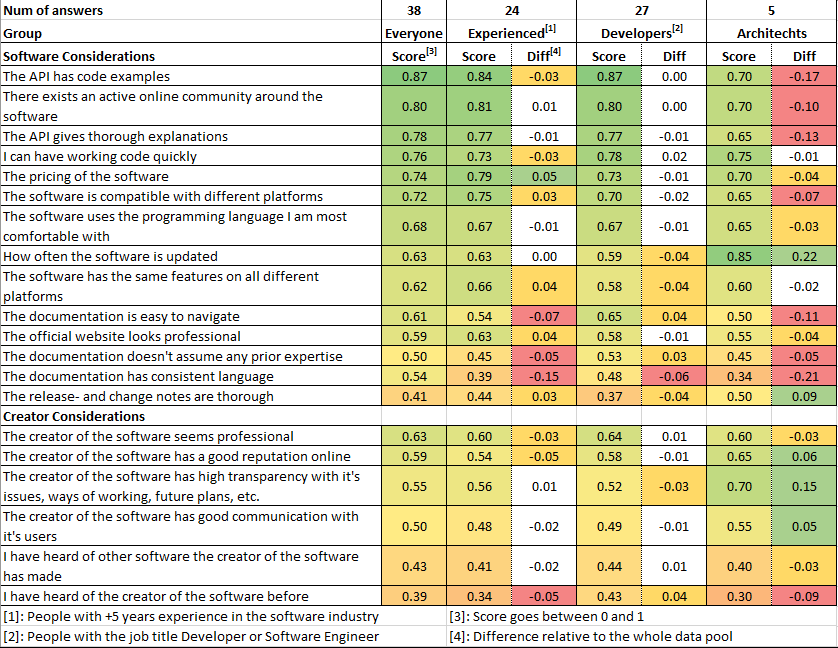
\includegraphics[width=\linewidth]{ScoresByPoints.png}
\caption{Caption}
\label{fig:scopresByPoints}
\end{figure}

\subsubsection{Creator behind the software factors}

Overall, the creator behind the software seem to be not non-important,
but not very important, with all factors scoring close to 0/10. The most
commonly considered factor was that the creator seemed professional, but
that only ranked 3.0/10. The least considered factor was 'I have heard of
the creator of the software before', which ranked -2.47/10.

With the more experienced users, they considered all factors even more
rarely than the control group, apart form transparency, which rose
slightly. Still, the scores are close to 0, and the creator once again
seem to be a somewhat important factor.

With the group consisting of only developers, it's much the same as
before, with the one exception that 'I have heard of the creator of the
software before' had an increase by 10\%. It is however still the least
considered factor.


\subsubsection{Conclusions from survey}

The two factors 'The documentation has consistent language' and 'The
release- and change notes are thorough' scored surprisingly low. This
goes against the literature. A potential difference could be that
question only states what would make the user *try* a new software. It
may not be an initial stopper, but could cause issues once the user has
decided to use the software. The follow-up interview indicated that so
may be the case. This will have to be investigated more.

The non-developer group cares about other things than the developers.
This groups includes consultants, directors, managers and architects.
These are positions in which they have power to make major decisions in
the company. The group therefor have other priorities than the lone
developer, that only considers his own workflow. In the next survey we
will make the context more specific so that the two groups are not mixed
up.

\subsection{Survey 2 Results}.
There are many ways you can view the results
We got 39 responses in total. The results were loaded into Qlik Sense
where we could find different groups and patterns. We looked at the
results from three angels: The overall average result, result depending
on your job title and result depending on how much experience you have
in the industry.
\\ \\
The job titles were divided into four groups: Architects, Developer and
Engineers, Managers and Other. The quantity and percentage of total can
be seen in the table \ref{tabl:jobs}.

\begin{table}[H]
\centering
\begin{tabularx}{\columnwidth}{r l l}
\textbf{Grouped Job Titles} &    \textbf{\# of answers} &     \textbf{\% of total} \\\hline
Architects              & 10           & 25.6\%  \\ \hline
Developer and Engineers & 21           & 53.8\%  \\\hline
Managers                & 4            & 10.3\%  \\\hline
Other                   & 4            & 10.3\%  \\\hline
\end{tabularx}
\caption{Main survey responses grouped by job titles}
\label{tabl:jobs}
\end{table}

Below we can see all the aspects, what points each job title gave it and
it's rank.

\begin{table}[H]
\centering
\begin{tabular}{r|l}
\textbf{Aspect ID} & \textbf{Aspect} \\ \hline
1   & How often the software is updated                                         \\
2   & I can have working code quickly                                           \\
3   & The API documentation gives thorough explanations on how it works         \\
4   & The API has code examples                                                 \\
5   & The documentation doesn't assume any prior expertise                      \\
6   & The documentation has consistent language                                 \\
7   & The documentation is easy to navigate                                         \\
8   & The official website looks professional\\
9   & The pricing of the software\\
10  & The release- and change notes are thorough\\
11  & The software has the same features on all different platforms\\
12  & The software is compatible with different platforms\\
13  & The software is offered in more than one programming language\\
14  & The software is open source\\
15  & The software uses the programming language I am most comfortable with\\
16  & There exists an active online community around the software\\ \hline
\end{tabular}
\caption{Question ID and questions}
\label{tab:questionID}
\end{table}

\begin{table}[H]
\centering
\begin{tabular}{|c|c:c|c:c|c:c|c:c|c:c|} \hline

\rotatebox{90}{Aspect ID}                                & \rotatebox{90}{Everyone Rank} & \rotatebox{90}{Avg Everyone} & \rotatebox{90}{Architects Rank} &\rotatebox{90}{Architects Score} & \rotatebox{90}{Dev\&Eng Rank} & \rotatebox{90}{Devs\&Eng Score} &  \rotatebox{90}{Man Rank} & \rotatebox{90}{Managers Score} & \rotatebox{90}{Other Rank} & \rotatebox{90}{Other Score}\\ \hline
4                                             &             1 & 0.90         &         1 &   0.92       &            1 & 0.91       &        1 & 0.79     &        1-2 & 0.94  \\ \hline
3     &             2 & 0.82         &         3 &   0.82       &            2 & 0.87       &        3 & 0.73     &          4 & 0.74  \\ \hline
2                                       &             3 & 0.80         &         2 &   0.85       &            4 & 0.80       &      4-5 & 0.71     &        1-2 & 0.94  \\ \hline
9                                           &             4 & 0.80         &         5 &   0.76       &            3 & 0.84       &        2 & 0.75     &          3 & 0.85  \\ \hline
15 &             5 & 0.68         &         6 &   0.69       &            5 & 0.73       &      6-7 & 0.63     &          5 & 0.69  \\ \hline
14                                           &             6 & 0.68         &         4 &   0.77       &            6 & 0.69       &        8 & 0.60     &          8 & 0.58  \\ \hline
16           &             7 & 0.65         &         8 &   0.63       &            7 & 0.67       &     9-11 & 0.54     &          6 & 0.65  \\ \hline
7                                 &             8 & 0.60         &         7 &   0.66       &            8 & 0.61       &       12 & 0.52     &         10 & 0.52  \\ \hline
8                               &             9 & 0.60         &         9 &   0.63       &           10 & 0.56       &      4-5 & 0.71     &         12 & 0.44  \\ \hline
12                   &            10 & 0.58         &        10 &   0.58       &           11 & 0.52       &     9-11 & 0.54     &          7 & 0.59  \\ \hline
1                                    &            11 & 0.58         &        11 &   0.52       &            9 & 0.57       &      6-7 & 0.63     &         11 & 0.51  \\ \hline
5                  &            12 & 0.47         &        13 &   0.47       &           13 & 0.44       &     9-11 & 0.54     &          9 & 0.52  \\ \hline
11         &            13 & 0.46         &        14 &   0.41       &           12 & 0.45       &    13-15 & 0.44     &         13 & 0.42  \\ \hline
6                             &            14 & 0.41         &        12 &   0.49       &           14 & 0.34       &       16 & 0.42     &         14 & 0.39  \\ \hline
13         &            15 & 0.36         &        15 &   0.37       &           15 & 0.31       &    13-15 & 0.44     &         16 & 0.23  \\ \hline
10                            &            16 & 0.33         &        16 &   0.26       &           16 & 0.29       &    13-15 & 0.44     &         15 & 0.35  \\ \hline
\end{tabular}
\caption{Caption}
\label{tab:my_label}
\end{table}


\subsubsection{Overall Result}
Overall, there were quite a lot of interesting finding when analyzing the results from the main survey.
In general, people are more likely to consider things when they are choosing for
a group rather than for themselves. For the three categories, Single is the
closest to the average result, with Group and Hobby existing as
opposites on either side of Single. In all but one case, if it's often
considered when choosing for a group, it's \textit{not} often considered when choosing
for a hobby project, and vice versa.

For the part of the survey regarding DX and people's feelings around software platforms, it can be said that there is a direct correlation between if an aspect in it's good form has a positive impact, that same aspect in it's
bad form will have about the same level of negative impact.
However, in all but once case, the positive effect is greater than the negative
effect, if only slightly. In general it is closely related to how often
something is considered. That is to say, if something will cause someone to have a non-neutral feeling regarding an aspect, they will also consider it when choosing a platform. Ergo, there is no uncoupling between what causes them to have a good DX, and what they consider when choosing a platform. There are some
outliers to this, but that is the general case.

The top three most considered aspects for each context can be seen in
the table \ref{tabl:top3}.

\begin{table}[H]
\centering
\begin{tabular}{r l}
\hline\hline
\multicolumn{2}{c}{\textbf{Average}} \\ \hline
1 &The API has code examples \\
2 & The API documentation gives thorough explanations on how it works \\
3 &I can have working code quickly \\
\hline\hline
\multicolumn{2}{c}{\textbf{Group}} \\ \hline
1 & The API has code examples                                        \\
2 & The API documentation gives thorough explanations on how it works \\
3 & The software is compatible with different platforms              \\
\hline\hline
\multicolumn{2}{c}{\textbf{Single}} \\ \hline
1 &  The API has code examples                                         \\
2 &  The API documentation gives thorough explanations on how it works  \\
3 &  I can have working code quickly                                   \\
\hline\hline
\multicolumn{2}{c}{\textbf{Hobby}} \\ \hline
1 & The pricing of the software    \\
2 & The API has code examples       \\
3 & I can have working code quickly\\ \hline
\end{tabular}
\caption{Top 3 considered aspects by each context}
\label{tabl:top3}
\end{table}
The overall result concluded that \textit{the} most considered aspect overall
is 'The API has code examples'. For hobby, it's the second most
important aspect, losing the first place by only 0.03 points.
Further, good code
examples had the biggest positive impact on developer experience, and
bad code examples had the biggest negative impact on DX. The negative
impact if the examples are bad are not as extreme as the positive impact
is if they are good however. In conclusion, API examples are a key
factor for software platforms' quality.
\\ \\
The thoroughness of the documentation is also one of the most important
aspects, coming in as the second most important aspect for all
categories except for Hobby. The positive DX-impact is as big as the
negative one, and it's also reflected in that it's consideration points
are as high as the DX-impact points.
\\ \\
Having working code quickly is also in the top three for all but the
group category, where it's in fourth place. The positive DX-impact if
you can have working code quickly is slightly higher than the negative
DX-impact if it takes a long time before you have working code. The
positive impact is also stronger than if you compare it to how often
it's considered.
\\ \\
Having the software be compatible with different platforms is a big
divider. It's the third most important aspect for Group, but one the
least important aspects for Hobby, and somewhere in the middle for
Single. The positive impact is lower than how often it's considered, and
the negative DX-impact is even less. If you exclude the Group-category,
it places itself on average as the 11\textsuperscript{th} most important
aspect, out of 16.
\\ \\
The pricing of the software is important to everyone, placing itself on
average as the 4\textsuperscript{th} most important aspect overall, but it is \textit{the}
most important aspect for Hobby. For group and single, it's both the
5\textsuperscript{th}  and 4\textsuperscript{th}  most important aspect respectively.

![consid_jobtitle2](./consid_jobtitle.png "Considerations grouped by different job titles")

There are several angles you can view this at. Here we discuss a few.

\subsubsection{Developer and Engineers compared with Architects}

For example, if we compare Architects and Developer and Engineers, they
are quite similar. On average, the score differences is 0.06. The
biggest difference for consideration questions is 'The documentation has
consistent language', where Architects average out at 0.49/1.00 in
points, making it 'Sometimes considered', whereas Developer and
Engineers only score 0.34/1.00, placing it between 'Sometimes consider'
and 'Rarely consider'. Their ranking does not differ much, with the
biggest ranking difference being two spots.

Below we can see the different aspects, sorted by average most
important, for Architects and Developers and Engineers.


\begin{table}[H]
\centering
\begin{tabularx}{\columnwidth}{X|c:c|c:c|c}

\textbf{Aspect}                                                    & \rotatebox{90}{\textbf{Architects Rank}}    &\rotatebox{90}{\textbf{Architects Score}} & \rotatebox{90}{\textbf{Dev\&Eng Rank}}  & \rotatebox{90}{\textbf{Devs\&Eng Score}}& \rotatebox{90}{\textbf{Diff}}\\ \hline
The API has code examples                                             &         1 & 0.92             &               1 & 0.91             & 0.01  \\ \hline
The API documentation gives thorough explanations on how it works     &         3 & 0.82             &               2 & 0.87             & 0.05  \\ \hline
The pricing of the software                                           &         5 & 0.76             &               3 & 0.84             & 0.08  \\ \hline
I can have working code quickly                                       &         2 & 0.85             &               4 & 0.80             & 0.05  \\ \hline
The software is open source                                           &         4 & 0.77             &               6 & 0.69             & 0.08  \\ \hline
The software uses the programming language I am most comfortable with &         6 & 0.69             &               5 & 0.73             & 0.05  \\ \hline
There exists an active online community around the software           &         8 & 0.63             &               7 & 0.67             & 0.03  \\ \hline
The documentation is easy to navigate                                 &         7 & 0.66             &               8 & 0.61             & 0.05  \\ \hline
The official website looks professional                               &         9 & 0.63             &              10 & 0.56             & 0.07  \\ \hline
The software is compatible with different platforms                   &        10 & 0.58             &              11 & 0.52             & 0.06  \\ \hline
How often the software is updated                                     &        11 & 0.52             &               9 & 0.57             & 0.05  \\ \hline
The software has the same features on all different platforms         &        14 & 0.41             &              12 & 0.45             & 0.04  \\ \hline
The documentation doesn't assume any prior expertise                  &        13 & 0.47             &              13 & 0.44             & 0.03  \\ \hline
The documentation has consistent language                             &        12 & 0.49             &              14 & 0.34             & 0.15  \\ \hline
The software is offered in more than one programming language         &        15 & 0.37             &              15 & 0.31             & 0.06  \\ \hline
The release- and change notes are thorough                            &        16 & 0.26             &              16 & 0.29             & 0.04  \\ \hline
\end{tabularx}
\caption{The ranking and scores of architects, compared with developers and engineers}
\label{tab:arch-devs}
\end{table}

\subsubsection{Architects compared with managers}

If we compare Architects and Managers, the differences are bit more
extreme. On average, they differ by 0.09 points. The biggest divider for
them is 'The release- and change notes are thorough', where they differ
by 0.18 points. The rank difference is only one spot though. Their
biggest dividers in rank differ by five spots. They are 'The official
website looks professional' and 'The documentation is easy to navigate'
where the first one is more important to Architects, and the second one
is more important to Managers.

\begin{table}[H]
\centering
\begin{tabularx}{\columnwidth}{X|c:c|c:c|c}

\textbf{Aspect}                                                    & \rotatebox{90}{\textbf{Architects Rank}}    &\rotatebox{90}{\textbf{Architects Score}} & \rotatebox{90}{\textbf{Manager Rank}}  & \rotatebox{90}{\textbf{Manager Score}}& \rotatebox{90}{\textbf{Diff}}\\ \hline
The API has code examples                                             &         1 & 0.92       &            1 & 0.79           & 0.13  \\ \hline
The API documentation gives thorough explanations on how it works     &         2 & 0.82       &          4-5 & 0.71           & 0.14  \\ \hline
The pricing of the software                                           &         3 & 0.76       &            3 & 0.73           & 0.09  \\ \hline
I can have working code quickly                                       &         5 & 0.85       &            2 & 0.75           & 0.01  \\ \hline
The software is open source                                           &         4 & 0.77       &            8 & 0.60           & 0.16  \\ \hline
The software uses the programming language I am most comfortable with &         6 & 0.69       &          6-7 & 0.63           & 0.06  \\ \hline
There exists an active online community around the software           &         9 & 0.63       &          4-5 & 0.71           & 0.08  \\ \hline
The documentation is easy to navigate                                 &         8 & 0.66       &         9-11 & 0.54           & 0.09  \\ \hline
The official website looks professional                               &         7 & 0.63       &           12 & 0.52           & 0.14  \\ \hline
The software is compatible with different platforms                   &        10 & 0.58       &         9-11 & 0.54           & 0.04  \\ \hline
How often the software is updated                                     &        11 & 0.52       &          6-7 & 0.63           & 0.11  \\ \hline
The software has the same features on all different platforms         &        13 & 0.41       &         9-11 & 0.54           & 0.07  \\ \hline
The documentation doesn't assume any prior expertise                  &        12 & 0.47       &           16 & 0.42           & 0.07  \\ \hline
The documentation has consistent language                             &        14 & 0.49       &        13-15 & 0.44           & 0.03  \\ \hline
The software is offered in more than one programming language         &        15 & 0.37       &        13-15 & 0.44           & 0.07  \\ \hline
The release- and change notes are thorough                            &        16 & 0.26       &        13-15 & 0.44           & 0.18  \\ \hline
\end{tabularx}
\caption{The ranking and scores of architects, compared with managers}
\label{tab:arch-devs}
\end{table}

\subsubsection{Developer and Engineers compared with Managers}

If we compare Developer and Engineer with Managers, we also find that
they're quite different. On average, they differ in points by 0.10
points. Their biggest differ in points is for 'The official website
looks professional', where they differ by 0.15 points, which is also
their biggest differ in ranking: 6 spots different.

\begin{table}[H]
\centering
\begin{tabularx}{\columnwidth}{X|c:c|c:c|c|}

\textbf{Aspect}                                                    & \rotatebox{90}{\textbf{Devs\&Eng Rank}}    &\rotatebox{90}{\textbf{Devs\&Eng Score}} & \rotatebox{90}{\textbf{Manager Rank}}  & \rotatebox{90}{\textbf{Manager Score}}& \rotatebox{90}{\textbf{Diff}}\\ \hline
The API has code examples                                             &               1 & 0.91       &            1 & 0.79           & 0.13  \\ \hline
The API documentation gives thorough explanations on how it works     &               2 & 0.87       &          4-5 & 0.71           & 0.14  \\ \hline
The pricing of the software                                           &               3 & 0.84       &            3 & 0.73           & 0.09  \\ \hline
I can have working code quickly                                       &               4 & 0.80       &            2 & 0.75           & 0.01  \\ \hline
The software is open source                                           &               5 & 0.73       &            8 & 0.60           & 0.16  \\ \hline
The software uses the programming language I am most comfortable with &               6 & 0.69       &          6-7 & 0.63           & 0.06  \\ \hline
There exists an active online community around the software           &               7 & 0.67       &          4-5 & 0.71           & 0.08  \\ \hline
The documentation is easy to navigate                                 &               9 & 0.57       &         9-11 & 0.54           & 0.09  \\ \hline
The official website looks professional                               &              10 & 0.56       &           12 & 0.52           & 0.14  \\ \hline
The software is compatible with different platforms                   &               8 & 0.61       &         9-11 & 0.54           & 0.04  \\ \hline
How often the software is updated                                     &              11 & 0.52       &          6-7 & 0.63           & 0.11  \\ \hline
The software has the same features on all different platforms         &              12 & 0.45       &         9-11 & 0.54           & 0.07  \\ \hline
The documentation doesn't assume any prior expertise                  &              13 & 0.44       &           16 & 0.42           & 0.07  \\ \hline
The documentation has consistent language                             &              14 & 0.34       &        13-15 & 0.44           & 0.03  \\ \hline
The software is offered in more than one programming language         &              15 & 0.31       &        13-15 & 0.44           & 0.07  \\ \hline
The release- and change notes are thorough                            &              16 & 0.29       &        13-15 & 0.44           & 0.18  \\ \hline
\end{tabularx}
\caption{The ranking and scores of architects, compared with developers and engineers}
\label{tab:arch-devs}
\end{table}


\subsubsection{Experience}

The responses were also divided into five groups, depending on how much
experience in the software industry the had. There were 5 people with
less than 5 years experience, 10 people with 5 - 10 years experience, 10
people with 10 - 15 years experience, 12 people with 15 - 25 years
experience and 2 people with 25+ years of experience in the software
industry.

\begin{table}[H]
\centering
\begin{tabularx}{\columnwidth}{X|c|c|c|c|c|c}
\textbf{Aspect}	&\textbf{\rotatebox{90}{	\<5 years	}}&\textbf{\rotatebox{90}{	5-10 years	}}&\textbf{\rotatebox{90}{	10-15 years	}}&\textbf{\rotatebox{90}{	15-25 years	}}&\textbf{\rotatebox{90}{	25+ years}}	\\ \hline
The API has code examples	&	0.91	&	0.93	&	0.89	&	0.85	&	1.00	\\ \hline
The API documentation gives thorough explanations on how it works	&	0.91	&	0.86	&	0.87	&	0.72	&	0.83	\\ \hline
I can have working code quickly	&	0.79	&	0.86	&	0.82	&	0.77	&	0.92	\\ \hline
The pricing of the software	&	0.73	&	0.86	&	0.81	&	0.83	&	0.67	\\ \hline
The software uses the programming language I am most comfortable with	&	0.68	&	0.73	&	0.68	&	0.74	&	0.50	\\ \hline
The software is open source	&	0.67	&	0.62	&	0.74	&	0.71	&	0.67	\\ \hline
There exists an active online community around the software	&	0.84	&	0.53	&	0.73	&	0.55	&	0.75	\\ \hline
The documentation is easy to navigate	&	0.60	&	0.68	&	0.64	&	0.48	&	0.71	\\ \hline
The official website looks professional	&	0.53	&	0.67	&	0.54	&	0.59	&	0.50	\\ \hline
How often the software is updated	&	0.66	&	0.52	&	0.52	&	0.58	&	0.50	\\ \hline
The software is compatible with different platforms	&	0.41	&	0.54	&	0.59	&	0.57	&	0.54	\\ \hline
The documentation doesn't assume any prior expertise	&	0.43	&	0.57	&	0.50	&	0.39	&	0.50	\\ \hline
The software has the same features on all different platforms	&	0.28	&	0.42	&	0.53	&	0.45	&	0.29	\\ \hline
The documentation has consistent language	&	0.41	&	0.45	&	0.40	&	0.32	&	0.58	\\ \hline
The software is offered in more than one programming language	&	0.28	&	0.35	&	0.35	&	0.36	&	0.25	\\ \hline
The release- and change notes are thorough	&	0.26	&	0.34	&	0.33	&	0.30	&	0.25	\\ \hline
\end{tabularx}
\caption{The ranking and scores of architects, compared with developers and engineers}
\label{tab:arch-devs}
\end{table}
\subsubsection{Decision Makers}

We divided the group into decision makers and non-decision makers. The
groups are of comparable size: There are 22 decision makers for groups
and 14 non-decision makers for groups, and 3 who answered that it is not
applicable. The following are the top three most important aspects to
the groups:

\begin{table}[H]
\centering
\begin{tabularx}{\columnwidth}{X|c:c|c:c|}
\textbf{Aspect}	&\textbf{\rotatebox{90}{DM* Rank}}&\textbf{\rotatebox{90}{DM* Score}}&\textbf{\rotatebox{90}{NDM** Rank}}&\textbf{\rotatebox{90}{NDM** Score}}	\\ \hline
The API has code examples	&	1	&	0.91	&	1	&	0.86	\\ \hline
The API documentation gives thorough explanations on how it works	&	2-3	&	0.83	&	3	&	0.80	\\ \hline
I can have working code quickly	&	2-3	&	0.83	&	4	&	0.79	\\ \hline
The pricing of the software	&	4	&	0.80	&	2	&	0.83	\\ \hline
The software uses the programming language I am most comfortable with	&	6	&	0.69	&	6	&	0.74	\\ \hline
The software is open source	&	5	&	0.70	&	8	&	0.63	\\ \hline
There exists an active online community around the software	&	7	&	0.62	&	5	&	0.75	\\ \hline
The documentation is easy to navigate	&	8	&	0.59	&	7	&	0.66	\\ \hline
The official website looks professional	&	9	&	0.58	&	9-10	&	0.61	\\ \hline
How often the software is updated	&	11	&	0.53	&	9-10	&	0.61	\\ \hline
The software is compatible with different platforms	&	10	&	0.55	&	12	&	0.54	\\ \hline
The documentation doesn't assume any prior expertise	&	12	&	0.45	&	11	&	0.60	\\ \hline
The software has the same features on all different platforms	&	13	&	0.43	&	14	&	0.46	\\ \hline
The documentation has consistent language	&	14	&	0.38	&	13	&	0.50	\\ \hline
The software is offered in more than one programming language	&	15	&	0.32	&	15	&	0.38	\\ \hline
The release- and change notes are thorough	&	16	&	0.29	&	16	&	0.35	\\ \hline  \hline
\multicolumn{5}{l}{*DM: Decision Makers, **NDM: Non-Decision Makers}
\end{tabularx}
\caption{Caption}
\label{tab:my_label}
\end{table}

It could also be interesting to see who the decision makers are. Divided
by job title and level, it looks like this:

\begin{table}[H]
\centering
\begin{tabular}{l l l l}
\textbf{Job Title} & \textbf{Level} & \textbf{DM*} & \textbf{NDM**} \\ \hline
Architect               & Middle & 0               & 0                   \\
Architect               & Senior & 7               & 2                   \\ \hline
Developer and Engineers & Middle & 3               & 4                   \\
Developer and Engineers & Senior & 5               & 7                   \\ \hline
Managers                & Middle & 1               & 0                   \\
Managers                & Senior & 3               & 0                   \\ \hline
Other                   & Middle & 0               & 0                   \\
Other                   & Senior & 3               & 1                   \\ \hdashline
&        &     \textbf{22}          & \textbf{14}              \\ \hline\hline
\multicolumn{4}{l}{*DM: Decision Makers, **NDM: Non-Decision Makers}

\end{tabular}
\caption{Caption}
\label{tab:my_label}
\end{table}

As we can see, and not surprising, all managers are decision makers.
Somewhat more interesting, two architects claim they are not in a
position to make decisions on what software others will use. We also see
that 50\% of Middle level people are decision makers, and 64\% of Senior
level people are decision makers.


\subsubsection{Compared to Survey 1}

The sample size is almost exactly the same in the two surveys. The first
survey had 38 responses, whereas the second one had 39. There are two
major differences between the two surveys. The first one had mostly just
Developer and Engineers, 74\%, only one manager, 3\%, and just five
architects, 13\%. As a reminder, the second survey had 53.8\% developer
and engineers, 10.3\% managers and 25.6\% architects. The second
difference is that in the second survey, the people were given a context
for when they were considering the aspects.

If we compare it to the first survey, we see some anomalies. To be able
to compare the rankings, we will exclude the two newly added questions
in this part. An interesting difference is the rank of 'The software is
compatible with different platforms'. However, this aspect is very
divided in the second survey depending on the situation. The rankings
for this aspect look as following: Group ranks it as the third most
important, whereas single ranks is at the 10\textsuperscript{th} spot and finally hobby at
place number 13. Similarly, the question 'The software has the same
features on all different platforms' has a big point difference when
comparing the first and second survey. However, this is also a divided
question depending on situation in the second survey. It's ranked by
Group at \#9, Single is tied between the 11\textsuperscript{th} and 12\textsuperscript{th} spot and for Hobby
it's #13. In the first survey, it's ranked as the #9 out of 14. The
change in ranking in both these cases can therefor somewhat be explained
by no context was given in the first survey.

But maybe most interesting is that in the first survey, 'There exists an
active online community around the software' ranked as the second most
important aspect, but is on average ranked as the sixth most important
aspect in the second survey. There is no difference on the context here,
in the second survey it's ranked at #6 by both Single and Hobby, and is
tied between 6th and 7th spot for Group. It \textit{is} slightly more important
for Developer and Engineers, but only by 0.04 points, so the fact that
the first survey had them as a majority cannot explain this either.
There does not seem to be any obvious explanation for this shift.

Below we can see the average result from the two surveys, with the
rankings. The two questions that don't exist in the first survey have
been excluded, and the ranking for the second survey recalculated.

\begin{table}[H]
\centering
\begin{tabularx}{\columnwidth}{X|c:c|c:c|c:c|}
\textbf{Aspect} & \textbf{\rotatebox{90}{S2* Rank}}&\textbf{\rotatebox{90}{S2* Points}}&\textbf{\rotatebox{90}{S1** Rank}}&\textbf{\rotatebox{90}{S1** Points}}&\textbf{\rotatebox{90}{Difference Points}} & \textbf{\rotatebox{90}{Difference Rank}} \\ \hline
The API has code examples                                             &                        1 & 0.90                      &                        1 & 0.87                       &       +0.03 &         0    \\ \hline
The API documentation gives thorough explanations [on how it works] &                        2 & 0.82                      &                        3 & 0.78                       &       +0.05 &        +1    \\ \hline
I can have working code quickly                                       &                        3 & 0.80                      &                        4 & 0.76                       &       -0.04 &        +1    \\ \hline
The pricing of the software                                           &                        4 & 0.80                      &                        5 & 0.74                       &       +0.06 &        +1    \\ \hline
The software uses the programming language I am most comfortable with &                        5 & 0.68                      &                        7 & 0.68                       &        0.00 &        +2    \\ \hline
\sout{The software is open source}                                    &                        - & 0.68                      &                        - & -                          &           - &         -    \\ \hline
There exists an active online community around the software           &                        6 & 0.65                      &                        2 & 0.80                       &       -0.15 &        -4    \\ \hline
The documentation is easy to navigate                                 &                        7 & 0.60                      &                       10 & 0.61                       &        0.00 &        +3    \\ \hline
The official website looks professional                               &                        8 & 0.60                      &                       11 & 0.59                       &       +0.01 &        +3    \\ \hline
The software is compatible with different platforms                   &                        9 & 0.58                      &                        6 & 0.72                       &       -0.14 &        -3    \\ \hline
How often the software is updated                                     &                       10 & 0.58                      &                        8 & 0.63                       &       -0.05 &        -2    \\ \hline
The documentation doesn't assume any prior expertise                  &                       11 & 0.47                      &                       12 & 0.50                       &       -0.03 &        +1    \\ \hline
The software has the same features on all different platforms         &                       12 & 0.46                      &                        9 & 0.62                       &       -0.16 &        -3    \\ \hline
The documentation has consistent language                             &                       13 & 0.41                      &                       13 & 0.45                       &       -0.04 &         0    \\ \hline
\sout{The software is offered in more than one programming language}  &                        - & 0.36                      &                        - & -                          &           - &              \\ \hline
The release- and change notes are thorough                            &                       14 & 0.33                      &                       14 & 0.41                       &       -0.09 &         0    \\ \hline \hline
\multicolumn{7}{l}{*S2: Survey 2, **S1: Survey 1}
\end{tabularx}
\caption{Caption}
\label{tab:my_label}
\end{table}

\subsubsection{Not considered}

Because of the way the data pool was shaped, we did not look at two
groups, which could have been interesting. The first one is company
size. 30 out of 39 people worked in companies with more than 1000
people, and only 4 out of 39 people worked in companies with less than
100 people. Therefor the data pool is too small to make any larger
claims on patterns.

The other group that could have been interesting to look at is the
professional level of the persons. However, 77\% were senior level, and
23\% were middle, and no one was junior level. The job title level is
somewhat arbitrary, and it can be argued that looking at years of
experience, where the answers are more divided, can substitute this
angle. Most of the people with a middle level have worked \< 5 years.
How big part of the work experience group are made up of middle and
senior level respectively can be seen in the table below.

\begin{table}[H]
\centering
\begin{tabular}{|l|l|l|}
\hline
\textbf{Years of experience} & \text{Middle level} & \textbf{Senior level} \\ \hline
\< 5 years           & 100\%         & 0\%           \\ \hline
5-10 years        & 20\%          & 80\%          \\ \hline
10-15 years       & 20\%          & 80\%          \\ \hline
15-25 years       & 0\%           & 100\%         \\ \hline
25+ years           & 0\%           & 100\%         \\ \hline
\end{tabular}
\caption{Caption}
\label{tab:my_label}
\end{table}

\subsection{Interview Results}

All of the interviews can be found in their full form in appendix X. In this section however
we will discuss some interesting findings in the interviews.

\subsubsection{API Documentation and Examples}

Just like the surveys suggested, API documentation and examples are very important
to everyone. It turns out that API examples are actually the first thing people
look for when encountering new documentation. All the interview subjects, when
encounter with the question "AB1 - When you look at API documentation, what are you usually looking for?"
answered in some shape or form that they first of all look for examples.

More text here...

\subsubsection{Release note}

More text here...

\subsubsection{Online Communities}

More text here...

\subsection{Evaluation of Qlik Core}


\section{Discussion and Conclusions}
\subsection{Surveys}
\subsection{Interviews}
\subsection{List of Recommendations for Software Platforms}
\subsection{Evaluation of Qlik Core}

\section{Acknowledgements}


\bibliographystyle{unsrt}
\bibliography{references}
\end{document}
